\subsection{Tenant \& subtenant relationship}
\label{sec:application:building_the_model:tenant_subtenant_relationship}

In the fourteenth step, another relationship between two objects is introduced. For this relation, a object of $.\type{Tenant}$ may reference a single $.\type{Tenant}$ object. \cref{subsec:library_of_transformations:type_level_transformations:nullable_class_fields} is used to introduce the field on the type level, while on the instance level, \cref{subsec:library_of_transformations:instance_level_transformations:nullable_class_field_values} is used to introduce the values.

The $classtype$ of the new field is $.\type{Tenant}$, as the field will be defined for tenants. The $name$ of the new field is $\type{subtenant}$ and the $fieldtype$ is equal to the $classtype$, $.\type{Tenant}$. The set of objects that will receive a value is defined as $valobjects = \{Tenant4\}$, while the set of objects that will not receive a value is defined as $nilobjects = \{Tenant1, Tenant2, Tenant3, Tenant5\}$. The union of these sets is equal to all the tenant objects, as expected. The function for $obids$ returns the existing identifier of each of these objects. The $values$ function is defined as follows:
\begin{align*}
    values = \{&(Tenant4, Tenant5)
\end{align*}

For the objects referenced by the objects in $valobjects$, the function $obids$ returns their existing identifier. The following model is obtained:

\LTXtable{\textwidth}{tex/06_application/02_building_the_model/tables/14_tenant_subtenant_relationship.tex}

\begin{figure}[p]
    \centering
    \begin{subfigure}{0.98\textwidth}
        \centering
        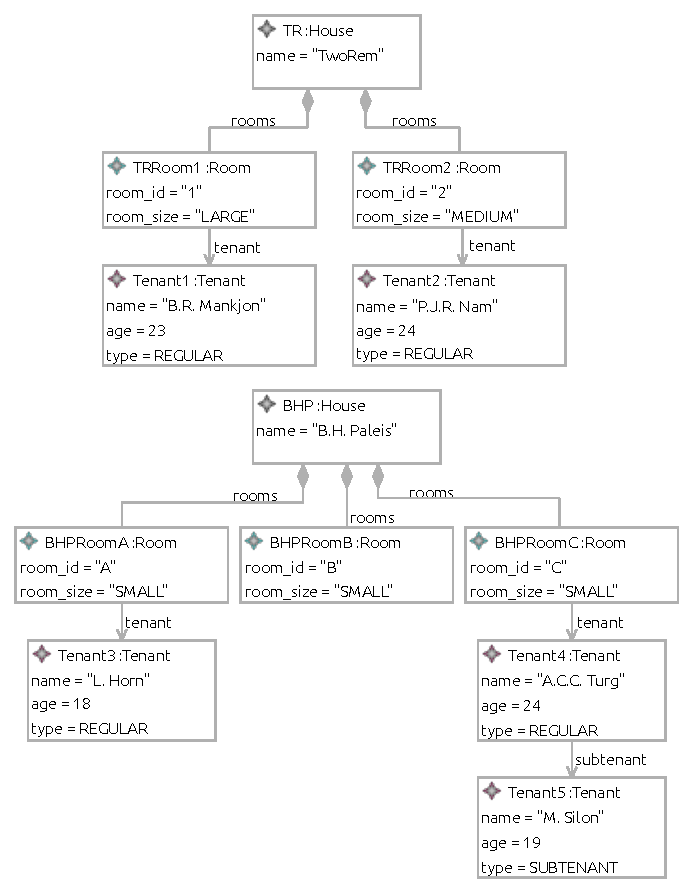
\includegraphics{images/06_application/instance_model/step14.pdf}
        \caption{Instance Model $Im_{14}$}
        \label{fig:application:building_the_model:tenant_subtenant_relationship:ecore:instance_model}
    \end{subfigure}
    \\
    \begin{subfigure}{0.98\textwidth}
        \centering
        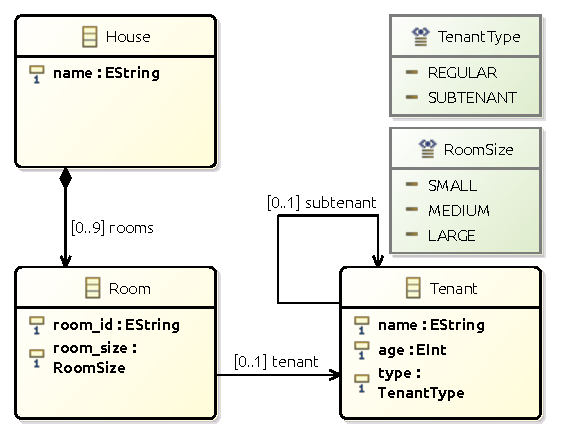
\includegraphics{images/06_application/type_model/step14.pdf}
        \caption{Type Model $Tm_{14}$}
        \label{fig:application:building_the_model:tenant_subtenant_relationship:ecore:type_model}
    \end{subfigure}
    \caption{The Ecore model after step 14}
    \label{fig:application:building_the_model:tenant_subtenant_relationship:ecore}
\end{figure}

\begin{figure}[p]
    \centering
    \begin{subfigure}{0.98\textwidth}
        \centering
        % To use this figure in your LaTeX document
% import the package groove/resources/groove2tikz.sty
%
\begin{tikzpicture}[scale=\tikzscale,name prefix=step14-]
\node[type_node] (n0) at (0.740, -0.400) {\ml{\textbf{House}\\name: \textbf{string}}};
\node[type_node] (n1) at (0.730, -1.585) {\ml{\textbf{Room}\\room\_id: \textbf{string}}};
\node[type_node] (n2) at (2.380, -0.560) {\ml{\textbf{RoomSize}\\\textit{LARGE}\\\textit{MEDIUM}\\\textit{SMALL}}};
\node[type_node] (n3) at (2.500, -1.590) {\ml{\textbf{Tenant}\\age: \textbf{int}\\name: \textbf{string}}};
\node[abstract_node] (n4) at (4.710, -0.980) {\ml{\textit{\textbf{TenantType}}}};
\node[type_node] (n5) at (3.810, -0.320) {\ml{\textbf{TenantType\$REGULAR}}};
\node[type_node] (n6) at (5.680, -0.320) {\ml{\textbf{TenantType\$SUBTENANT}}};

\path[basic_edge, composite](n0.south -| 0.730, -1.585) -- node[lab] {\ml{rooms}} (n1) ;
\path[basic_edge] (n1)  -- node[lab] {\ml{room\_size}} (n2) ;
\path[basic_edge] (n3)  -- node[lab] {\ml{type}} (n4) ;
\path[basic_edge](n1.east |- 2.500, -1.590) -- node[lab] {\ml{tenant}} (n3) ;
\path[basic_edge] (n3)  -- (3.430, -2.140) --  (n3) 
node[lab] at (3.430, -2.140) {\ml{subtenant}};
\path[subtype_edge] (n6)  --  (n4) ;
\path[subtype_edge] (n5)  --  (n4) ;
\end{tikzpicture}

        \caption{Instance Graph $IG_{14}$}
        \label{fig:application:building_the_model:tenant_subtenant_relationship:groove:instance_graph}
    \end{subfigure}
    \\
    \begin{subfigure}{0.98\textwidth}
        \centering
        % To use this figure in your LaTeX document
% import the package groove/resources/groove2tikz.sty
%
\begin{tikzpicture}[scale=\tikzscale,name prefix=step14-]
\node[type_node] (n0) at (0.740, -0.400) {\ml{\textbf{House}\\name: \textbf{string}}};
\node[type_node] (n1) at (0.730, -1.585) {\ml{\textbf{Room}\\room\_id: \textbf{string}}};
\node[type_node] (n2) at (2.380, -0.560) {\ml{\textbf{RoomSize}\\\textit{LARGE}\\\textit{MEDIUM}\\\textit{SMALL}}};
\node[type_node] (n3) at (2.500, -1.590) {\ml{\textbf{Tenant}\\age: \textbf{int}\\name: \textbf{string}}};
\node[abstract_node] (n4) at (4.710, -0.980) {\ml{\textit{\textbf{TenantType}}}};
\node[type_node] (n5) at (3.810, -0.320) {\ml{\textbf{TenantType\$REGULAR}}};
\node[type_node] (n6) at (5.680, -0.320) {\ml{\textbf{TenantType\$SUBTENANT}}};

\path[basic_edge, composite](n0.south -| 0.730, -1.585) -- node[lab] {\ml{rooms}} (n1) ;
\path[basic_edge] (n1)  -- node[lab] {\ml{room\_size}} (n2) ;
\path[basic_edge] (n3)  -- node[lab] {\ml{type}} (n4) ;
\path[basic_edge](n1.east |- 2.500, -1.590) -- node[lab] {\ml{tenant}} (n3) ;
\path[basic_edge] (n3)  -- (3.430, -2.140) --  (n3) 
node[lab] at (3.430, -2.140) {\ml{subtenant}};
\path[subtype_edge] (n6)  --  (n4) ;
\path[subtype_edge] (n5)  --  (n4) ;
\end{tikzpicture}

        \caption{Type Graph $TG_{14}$}
        \label{fig:application:building_the_model:tenant_subtenant_relationship:groove:type_graph}
    \end{subfigure}
    \caption{The GROOVE graphs after step 14}
    \label{fig:application:building_the_model:tenant_subtenant_relationship:groove}
\end{figure}

A visual representation of $Tm_{14}$ and $Im_{14}$ can be found in \cref{fig:application:building_the_model:tenant_subtenant_relationship:ecore}. Similarly, a visual representation of $TG_{14}$ and $IG_{14}$ can be found in \cref{fig:application:building_the_model:tenant_subtenant_relationship:groove}. Please note that because of the definitions of $f_{14}(Im_{14})$ and $f'_{14}(IG_{14})$, we have that $f_{14}(Im_{14}) = IG_{14}$ and $f'_{14}(IG_{14}) = Im_{14}$. Furthermore, $f_{14}(Im_{14})$ and $f'_{14}(IG_{14})$ are valid mapping functions themselves, such that they can be combined with another mapping function in the next step.

The visualisation shows once more a new field for referencing existing objects. The most important aspect of this field is that it can reference objects from the same type as its source type. This property is useful for making self relations, but also for creating relations between objects of the same type, as can be seen in the visualisation of $Tenant4$, which has $Tenant5$ as a subtenant.

\afterpage{\FloatBarrier}